\documentclass[11pt]{article}
\usepackage[a4paper,margin=24mm]{geometry}
\usepackage{amsmath,amssymb,booktabs,graphicx,hyperref,longtable}
\usepackage[T1]{fontenc}
\newcommand{\RobotMass}{0.500}
\newcommand{\CompletedRuns}{15}
\newcommand{\StandingHeight}{0.1358}
\newcommand{\StudyRuns}{12}
\newcommand{\StudyStatus}{completed short-budget exploratory study}

\title{A Reproducible PPO Pipeline for a Provisional Six-Joint Microduck Biped\\\large Preliminary Methods and Model-Validation Report}
\author{Microduck project}
\date{\today}
\begin{document}
\maketitle
\begin{abstract}
This report documents an executable pipeline for a user-supplied six-joint biped model. The central research question is how curriculum learning and physically consistent randomization affect locomotion reliability under a fixed local compute budget. The implementation uses MuJoCo, MuJoCo Warp, mjlab, and maintained RSL-RL PPO. Model masses, inertia tensors, and actuator ratings originate from an uncalibrated URDF and remain provisional. The model has total mass \RobotMass\ kg. A conservative standing diagnostic reaches a minimum base height of \StandingHeight\ m. The initial-study artifact index contains \CompletedRuns\ recorded training runs; their existence is not evidence of reliable walking. The independent study contains \StudyRuns\ policies. Its status is \StudyStatus. A separate futuristic-CAD and keyboard-control extension is reported with its own measured artifacts below. Hardware deployment and transfer performance are untested. This preliminary report separates verified engineering behavior from planned research claims.
\end{abstract}

\section{Scope and research question}
The project begins with an articulated URDF and a separate appearance-oriented CAD model. These inputs serve different purposes: the URDF defines kinematics and estimated rigid-body dynamics, whereas the redesigned CAD provides a visual design concept. No density-based mass extraction or joint-clearance validation is claimed for the CAD. The later futuristic extension imports the actual detailed surfaces and uses explicit provisional joint mappings and dynamics; importing appearance does not establish calibrated hardware dimensions.

The intended empirical question is: for this custom biped and a fixed local compute budget, how do a command curriculum and physically grounded domain randomization affect reliability and robustness? A new morphology with standard PPO is not an algorithmic novelty. This report describes the infrastructure needed to evaluate the question, records executed checks, and explicitly leaves absent experiments unmeasured.

\section{Related work and dependency contributions}
PPO introduces a clipped policy-gradient surrogate for repeated minibatch optimization \cite{ppo}. Generalized advantage estimation combines temporal-difference residuals with exponentially decaying weights \cite{gae}. Work on massively parallel locomotion demonstrates the utility of collecting many independent environments for a shared policy \cite{rudin}; results on its robots do not establish performance for this biped. mjlab supplies manager-based task composition and an integration with GPU physics \cite{mjlab}. MuJoCo supplies rigid-body dynamics \cite{mujoco}; MuJoCo Warp provides vectorized simulation \cite{mjwarp}, and RSL-RL supplies the maintained PPO implementation \cite{rsl}. The project-specific contributions are model auditing, task definition, terminal-observation handling, bounded orchestration, evaluation interfaces, and artifact linkage. Dynamics randomization studies motivate evaluating uncertain physical parameters \cite{randomization}; their transfer results do not establish transfer for this robot. No simulator or PPO implementation is presented as original work.

\section{Robot model and physical validation}
The supplied mechanism has a torso root, a fixed head, and two symmetric leg chains. Each leg has hip roll about the longitudinal axis, hip pitch about the lateral axis, and knee pitch about the lateral axis. Thigh, shin, and foot attachment joints are fixed. A free joint connects the torso to the world; the pelvis is not fixed during locomotion. Linear quantities use metres, masses use kilograms, and angles use radians. The authoritative joint order is left hip roll, left hip pitch, left knee, right hip roll, right hip pitch, right knee.

The importer reads explicit inertial origins, rotates inertia tensors into the link frame, and checks positive eigenvalues and principal-moment triangle inequalities. It preserves masses and link offsets, creates separate visual and collision primitives, and records the imported tree in a machine-readable audit. It supports the supplied primitive-box URDF and rejects unsupported geometry rather than silently guessing a representation. The baseline enables robot--terrain contact and disables self-collision. This exclusion is a limitation: large joint excursions require a separate self-collision audit before realistic locomotion claims.

Initial validation checks loading, joint-command directions away from position stops, a gravity drop, finite state, and a five-second standing controller. Standing uses the same floating-base geometry and provisional PD gains. A failed standing gate blocks training. A successful standing test establishes only a local equilibrium under one configuration; it does not establish perturbation recovery, dynamic stepping, or actuator realism.
\begin{figure}[ht]
\centering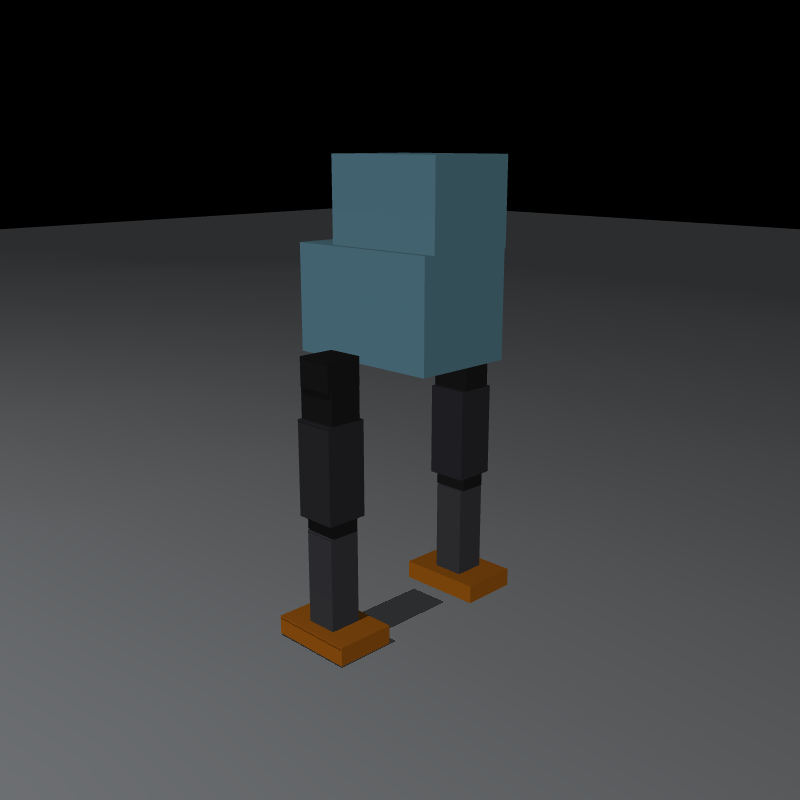
\includegraphics[width=.44\linewidth]{../results/figures/imported_robot.png}
\caption{Actual imported physical model. This primitive geometry is distinct from the appearance CAD.}
\end{figure}

\begin{figure}[ht]
\centering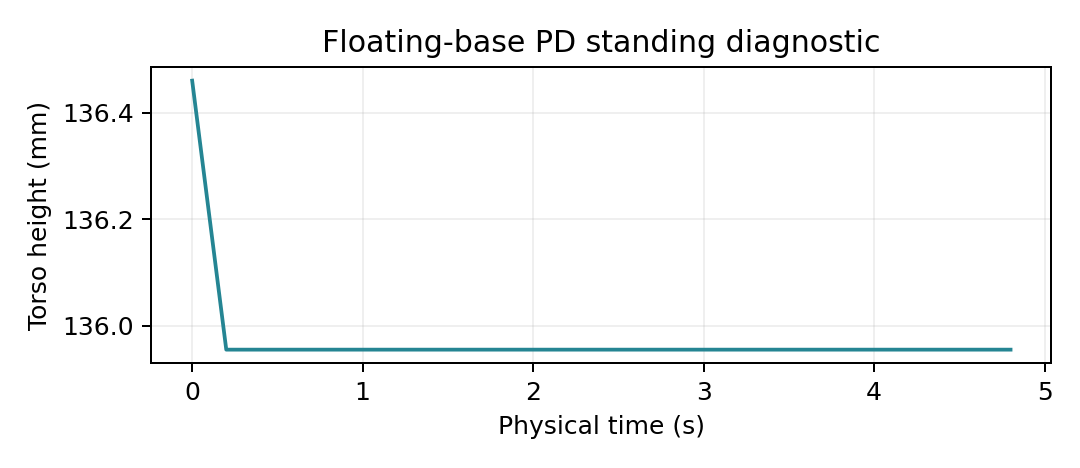
\includegraphics[width=.75\linewidth]{../results/figures/standing.png}
\caption{Measured torso height during the five-second standing diagnostic. This is a controller check, not a learned walking result.}
\end{figure}
\section{Task, observations, and control}
The initial task uses flat ground with commands for forward velocity and yaw rate. Lateral commands are zero in the first baseline because the small mechanism has no ankle joints. Episodes end at a configured time limit or on a low or tilted torso. Non-finite state raises an error and is not hidden as an ordinary fall. Training uses independent copies of one robot, with one shared actor and value function. Separate random seeds are separate trained policies, not environment indices.

\begin{table}[ht]\centering
\begin{tabular}{lrrl}\toprule
Field & Dimensions & Scale & Frame/units\\\midrule
Angular velocity &3&0.25&body, rad/s\\
Projected gravity &3&1&body, unit vector\\
Relative joint positions &6&1&rad\\
Joint velocities &6&0.05&rad/s\\
Previous bounded action &6&1&dimensionless\\
Velocity command &3&1&m/s, m/s, rad/s\\\bottomrule
\end{tabular}
\caption{Actor and critic share 27 proprioceptive inputs. No base linear velocity or contact ground truth is exposed to the actor. Orientation estimation and joint sensing remain deployment requirements.}
\end{table}

The actor outputs a diagonal-Gaussian latent action $u$. The environment deterministically maps it through $a=\tanh(u)$ and computes
\begin{align}
q^*&=\operatorname{clip}(q_0+s\odot a,q_{\min},q_{\max}),\\
\tau&=\operatorname{clip}(K_p\odot(q^*-q)-K_d\odot\dot q,-\tau_{\max},\tau_{\max}).
\end{align}
PPO stores the unsquashed latent action and evaluates its Gaussian log probability consistently. This is a policy over latent actions followed by a fixed actuator transformation; the optimizer does not apply Gaussian likelihoods to clipped joint targets. PD control is evaluated every physics step. The initial simulation step is 0.002 s, with ten substeps per 0.02 s policy step. Gains and effort limits are provisional; no measured hobby-servo dynamics or torque--speed envelope is asserted.

\section{Reward definition and curriculum}
Reward terms are rates multiplied by policy timestep before accumulation. Tracking uses an exponential squared planar error with bandwidth 0.025 m/s; yaw tracking has bandwidth 0.15 rad/s. A compact upright reward supplements tracking. Height shaping uses the nominal base height and a 0.018 m bandwidth. These values are hypotheses for this small morphology, not established optimum settings.

\begin{longtable}{lrl}
\toprule Term & Weight & Rate before weighting\\\midrule
Planar tracking &3&$\exp(-\|v_{xy}-c_{xy}\|^2/0.025^2)$\\
Yaw tracking &0.5&$\exp(-(\omega_z-c_z)^2/0.15^2)$\\
Upright &0.25&$\exp(-\|g_{xy}\|^2/0.2^2)$\\
Base height &0.1&$\exp(-((h-h_0)/0.018)^2)$\\
Vertical motion &$-2$&$v_z^2$\\
Roll/pitch speed &$-0.02$&$\|\omega_{xy}\|^2$\\
Torque squared &$-0.01$&$\sum_j\tau_j^2$\\
Joint speed &$-0.0002$&$\sum_j\dot q_j^2$\\
Action change &$-0.02$&$\|a_t-a_{t-1}\|^2$\\
Joint-limit excess &$-5$&sum of positive soft-limit excesses\\
Saturation &$-0.1$&fraction near torque bounds\\
Contact-conditioned slip &$-3$&sum of contacting foot planar speed squared\\
Non-foot contacts &$-2$&number of non-foot bodies touching ground\\\bottomrule
\end{longtable}
Terms with different physical dimensions are weighted dimensional costs; they are not all unitless physical quantities. Rates, units, weights, and timestep scaling are part of the frozen experiment definition. No explicit gait-phase signal is used. Foot-clearance and air-time shaping remain absent until a concrete gait failure justifies their introduction.

The command curriculum has three levels: standing, forward commands up to 0.03 m/s, then commands up to 0.06 m/s with yaw rates up to 0.15 rad/s. Promotion requires completed-episode survival exceeding 90\% of the time limit and mean tracking RMSE below 0.025 m/s; survival below 50\% triggers demotion. Changes and measured triggers are logged. Fixed-difficulty evaluation prevents promotions from appearing as misleading improvements in the test distribution.

Initial randomization includes friction, density-consistent mass/inertia perturbations, gains, sensor noise, and short control delay. Density scaling uses the framework's physically consistent pseudo-inertia operation. These small bounds are provisional uncertainty models. Measured center-of-mass uncertainty, actuator strength, external pushes, and modest terrain variation require additional calibration and validation; no robustness result on those factors is claimed here.

\begin{figure}[ht]\centering
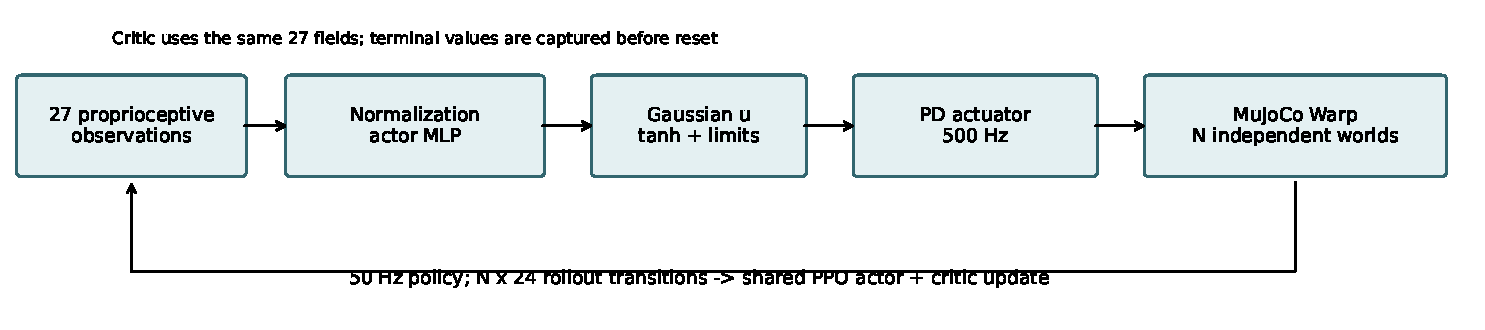
\includegraphics[width=.98\linewidth]{../results/figures/control_loop.pdf}
\caption{Configured control and learning loop. Parallel worlds share policy weights; independent research seeds use separate runs.}
\end{figure}
\section{PPO and timeout semantics}
Separate actor and critic MLPs use hidden widths 256, 256, and 128 with ELU activations. Empirical observation normalization is part of checkpoint and inference state. The starting Gaussian standard deviation is 0.5 in latent action units. The candidate PPO settings are $\gamma=0.99$, $\lambda=0.95$, learning rate $3\times10^{-4}$, five optimization epochs, four minibatches, entropy weight 0.01, value weight 1, and maximum gradient norm 1. The objective follows
\[
L^{\rm clip}=\mathbb E_t[\min(r_t\widehat A_t,\operatorname{clip}(r_t,1-0.2,1+0.2)\widehat A_t)].
\]
RSL-RL implements the optimization and rollout buffer. Its pinned implementation is inspected for advantage normalization and return handling instead of assuming all defaults match a paper.

Time-limit bootstrapping uses the post-action terminal observation before reset. For a pure timeout, the wrapper adds $\gamma V(s_{t+1}^{\rm terminal})$ to the terminal reward, then reports done to break the GAE recursion across episodes. A true fall takes precedence when a timeout and fall coincide, and receives no bootstrap. The upstream timeout hook is omitted to prevent adding the bootstrap twice. Reset observations become the next policy input only after the terminal value is captured.

\section{Compute protocol and reproducibility}
A rollout has $N\times24$ aggregate transitions, where $N$ is the number of environments. One policy step has ten physics substeps. PPO epochs, gradient steps, aggregate transitions, and updates are recorded separately. Simulator-only benchmarks exclude optimizer time; training metrics include rollout and optimization time with GPU synchronization at boundaries. Initialization and kernel compilation are reported separately. Environment count is selected from measured memory and throughput, rather than assuming thousands of replicas fit on a laptop.

Each run has an actual UTC timestamp and UUID, resolved configuration, asset and lockfile hashes, code revision and working-tree status, seed, hardware metadata, portable JSONL records, and TensorBoard output. Checkpoints include actor, critic, optimizer, normalization state, random number generators, curriculum level, and transition count. Training-state continuation resets physics; bitwise simulator restoration and GPU determinism are not promised. Export includes observation ordering, scaling, control frequency, and joint-target conventions. Numerical parity is required for the exported inference model.

\section{Evaluation and short-budget evidence}
The study is a matched $2\times2$ factorial comparison of curriculum and randomization, with seeds 0, 1, and 2 trained sequentially. Architecture, rewards, simulator, transition budget, and held-out evaluation sequences are held fixed. Without curriculum, commands span the final training distribution from the start. Equal-sample and equal-time comparisons answer different questions and must be reported separately.

Validation and test suites use disjoint episode seeds. Acceptance requires survival for at least 95\% of an episode, planar RMSE at most 0.025 m/s, yaw RMSE at most 0.1 rad/s, and no fall. This criterion is frozen before selecting policies. Episodes provide within-policy diagnostics; independent training seeds are the units for uncertainty on learning performance. Mechanical cost of transport uses positive absolute mechanical work divided by $mgd$ and excludes non-forward commands and forward distances below 0.02 m. This quantity is not measured battery energy. In the supplementary stopping diagnostic, a forward command switches to zero at five seconds; it is separate from checkpoint selection and the primary held-out comparison.

The initial study uses 1,536,000 aggregate transitions per policy with three training seeds per condition. Only final checkpoints are eligible; validation selects within that fixed eligible set. Training conditions share the transition budget, architecture, rewards and held-out cases. Study status: \textbf{\StudyStatus}.
\begin{table}[ht]\centering
\begin{tabular}{lrrr}\toprule
Condition & Seeds & Success (\%) & Planar RMSE (m/s)\\\midrule
baseline & 3 & 20.0 & 0.0284\\
curriculum & 3 & 20.0 & 0.0531\\
randomization & 3 & 20.0 & 0.0429\\
both & 3 & 20.0 & 0.0457\\
\bottomrule\end{tabular}

\caption{Held-out test aggregates generated from episode artifacts, averaged at the independent training-run level. Missing data remain visibly marked.}
\end{table}
\IfFileExists{../results/figures/test_success.png}{\begin{figure}[ht]\centering
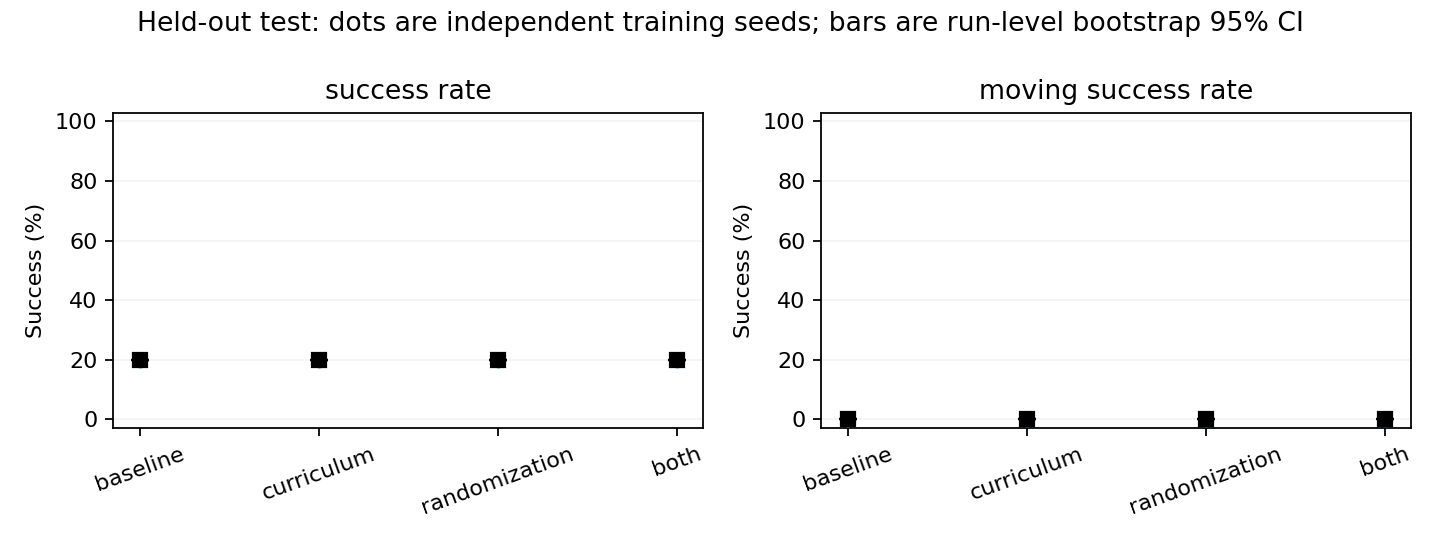
\includegraphics[width=.98\linewidth]{../results/figures/test_success.png}
\caption{Actual independent seeds and percentile bootstrap intervals from 10,000 resamples of run means (RNG seed 0). Episodes are not treated as independent trained policies.}\end{figure}}{}
\IfFileExists{../results/figures/learning.png}{\begin{figure}[ht]\centering
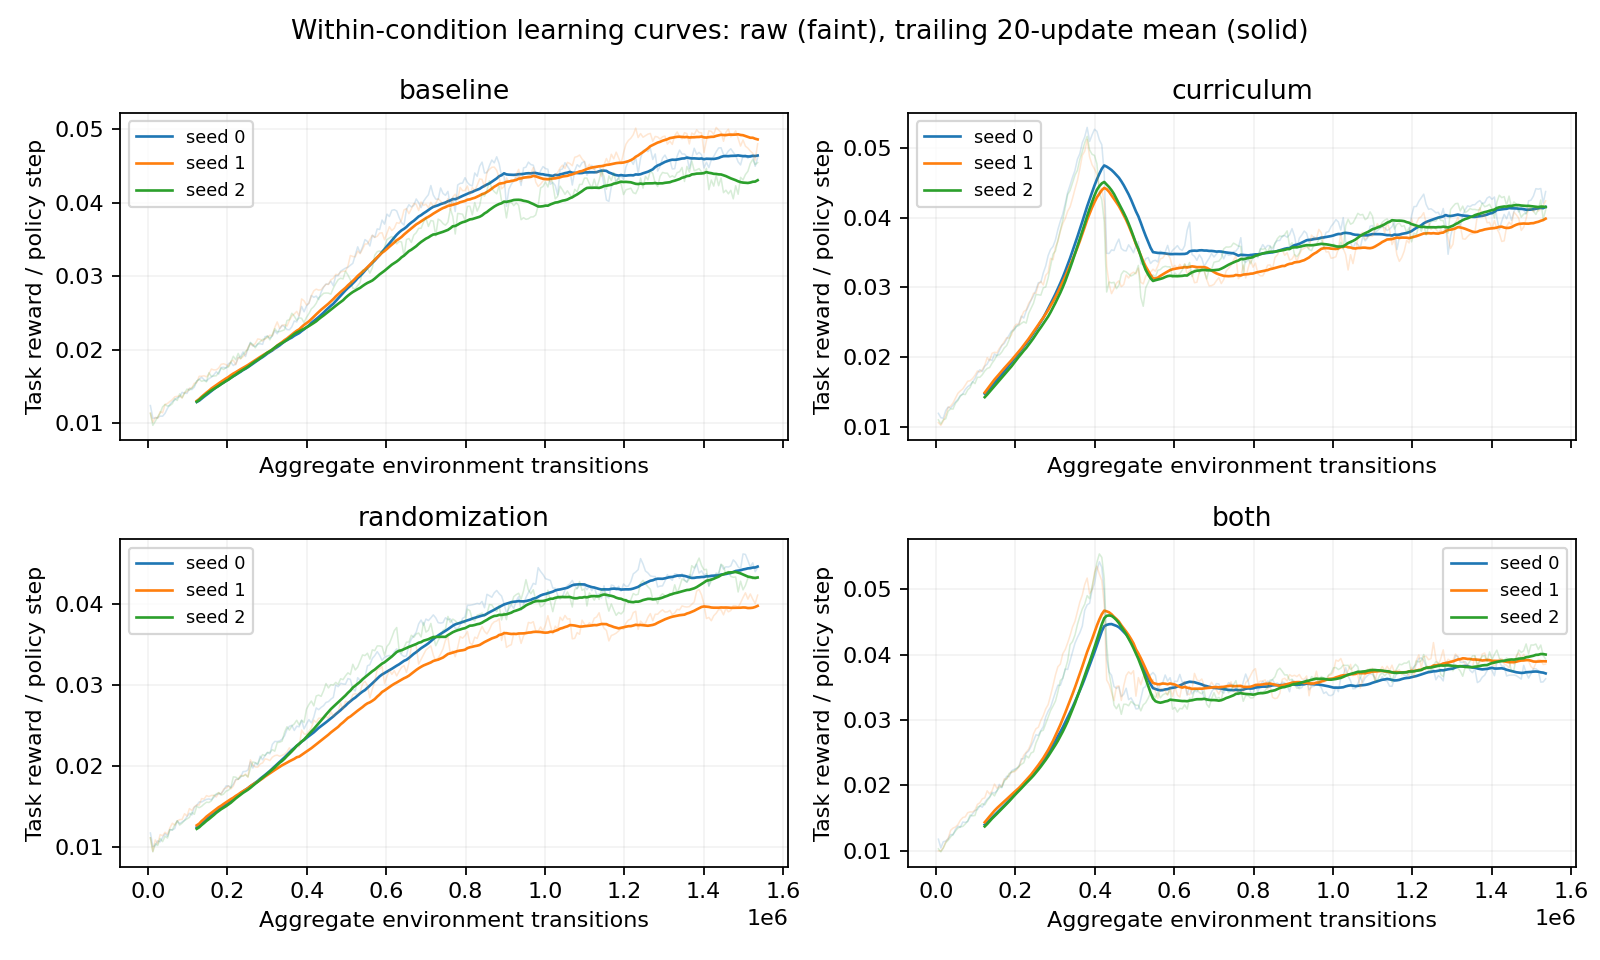
\includegraphics[width=.88\linewidth]{../results/figures/learning.png}
\caption{Actual per-update task reward, raw and trailing 20-update arithmetic mean. Curriculum changes difficulty, so comparisons of reliability use the fixed test suite rather than these rewards.}\end{figure}}{}
No policy passed the full moving-command acceptance criterion on the fixed held-out suite. Standing cases account for the observed aggregate successes. This does not imply an absence of forward displacement; heading error, speed error, or falls can each cause failure. The sample contains three independent training seeds per condition. Degenerate bootstrap intervals from identical seed outcomes do not establish certainty outside these sampled policies and test conditions. For the validation-selected policy, the 0.045 m/s command produced mean forward displacement 0.436 m and yaw-rate RMSE 0.468 rad/s over the corresponding held-out cases. Thus forward motion occurred, but heading control failed the declared criterion. 

\textbf{Terrain generalization, held-out mass/delay grids, and hardware transfer: NOT MEASURED.} The generated result manifest maps available model and run evidence to its source hashes. Missing experiments are not replaced with synthetic learning curves or fabricated confidence intervals. Raw curves, when present, are pipeline diagnostics and are not evidence of reliable locomotion.

\IfFileExists{futuristic_results.tex}{\section{Futuristic CAD and physical-transfer revision}
All 122 actual futuristic FreeCAD surfaces are imported into an explicit provisional six-joint assembly. The CAD hip, knee and ankle landmarks define its proportions and bent neutral pose. Estimated mass is 0.500 kg; actuator dynamics, mass properties, mechanical clearance and self-collision are not hardware-validated.

The earlier long run was stopped after validation and interactive use exposed poor backward heading, rough motion and transition failures. Good planar speed error did not establish command reliability. The replacement revision uses 41 observations: the earlier 29 plus applied-target and target-velocity state. A shared CPU/GPU controller ramps commands, filters complete motor targets, and limits target speed. A 1.5 Hz reference cadence with 8 mm lift replaces the faster reference. Extra yaw-error and complete-target velocity/acceleration costs address the reported failures. Left/right mirror consistency uses the maintained RSL-RL extension. Prior actor/critic mappings are retained by zero-padding the new input channels, with a tested fresh-optimizer weight transfer.

The new sensor-to-position runtime exactly matches simulator targets in a 100-step handoff check. The exported ONNX runtime loads without MuJoCo, mjlab or RSL-RL; it performs no hardware I/O. The 21 software checks include randomized GPU execution, reset isolation, target-rate bounds, observation migration, and mirror/gait consistency. Passing these checks is not walking acceptance.

The randomized 20,000-update training stage is in progress on the local RTX 4060. It varies physically consistent mass/inertia, friction, gains, effort, actuation delay, and gyro/encoder bias and noise. These ranges model uncertainty and are not calibrated servo measurements. Validation prioritizes the weakest command group and worst yaw error; held-out physical-parameter draws and CPU command transitions remain separate gates. The revised policy is not yet qualified for all commands. Actual servo identities, mass/COM, sensor feedback and timing are still needed; physical hardware performance remains unmeasured. The final artifact-linked tables will replace this progress section after the scheduled validation/test pipeline completes.
}{}

\section{Limitations, failure cases, and next gates}
The physical model is only a provisional URDF approximation. The futuristic extension uses CAD proportions in an assumed articulated assembly; it has not been calibrated against hardware. Missing manufacturer identities prevent claims about gear efficiency, motor heating, bus delay, backlash, or servo bandwidth. Self-collision is disabled in the initial baseline. The model has no independently controlled ankles, and its small support geometry restricts feasible motions. Saturation, contact stability, foot slip, and unintended body contacts require explicit review before escalating command ranges.

A conservative standing gate can pass while a learned controller falls immediately. Short PPO runs establish that gradients and checkpoints execute, not that a stable gait has emerged. The execution manifest records bounded pilot training, resumed continuation, fixed validation and export parity. Matched-study status is \StudyStatus; successful execution is not equivalent to reliable walking. Any failed run remains in the artifact index. Push, delay, mass, and terrain failure boundaries must be evaluated over predefined grids before robust locomotion can be claimed.

\section{Reproducibility statement and conclusion}
The project provides an isolated dependency lock, model audit, configuration files, CLI commands, tests, run manifests, and editable report sources. Reproduction begins with hardware diagnostics and model validation, proceeds through CPU and GPU smoke tests and a benchmark, and only then launches bounded training. Local artifacts are authoritative; GitHub publication is separate and must identify an actual remote and pushed commit. CAD ownership remains separate from code and dependency licensing. AI assistance was used in preparing implementation and prose; generated outputs require human review, especially before any hardware experiment.

The current deliverable is a reproducible engineering pipeline and preliminary empirical report. The short-budget study supports only the measured artifact-linked comparisons. Longer training and calibrated hardware experiments are required before broad locomotion or transfer conclusions. A policy export is an inference artifact and does not authorize operation on a physical robot.
\bibliographystyle{plain}\bibliography{references}
\end{document}
